\chapter{Vocabulaire de la théorie des ensembles}
\label{chap:ensembles}

\section{Les ensembles}

\begin{itemize}
    \item $E \to$ l'ensemble
    \item $\mathcal{P}(E) \to$ l'ensemble des parties de $E$ :
    \[\mathcal{P}(E) = \{A \mid A \subset E\}\]
\end{itemize}

\begin{exemple}
$E = \{a,b\}$, \quad $\mathcal{P}(E) = \{\emptyset, \{a\}, \{b\}, \{a,b\}\}$
\end{exemple}

\begin{itemize}
    \item $\subset \to$ inclusion : $A \subset B$ signifie $\forall x,\ (x \in A \implies x \in B)$
    \item $\in \to$ appartenance
\end{itemize}

\begin{center}
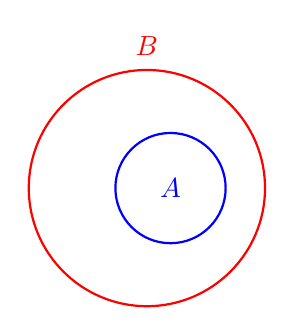
\begin{tikzpicture}
\draw[red, thick] (0,0) circle (1.5);
\node[red] at (0,1.8) {$B$};
\draw[blue, thick] (0.3,0) circle (0.7);
\node[blue] at (0.3,0) {$A$};
\end{tikzpicture}
\end{center}

\begin{prop}
\label{prop:card-parties}
Soit $E$ un ensemble fini,
\[\Card(\mathcal{P}(E)) = 2^{\Card(E)}\]
\end{prop}

\begin{proof}
Soit $E$ un ensemble fini, $|E| = n \in \mathbb{N}$.

$\dbinom{n}{k}$ : nombre de parties à $k$ éléments dans un ensemble à $n$ éléments.

Pour $k\in\inter{0}{n}$, notons $\mathcal{A}_k$ l'\emph{ensemble} des parties de $E$ à $k$ éléments :
\[\mathcal{A}_k = \{A \in \mathcal{P}(E) \mid |A| = k\}, \qquad \text{de sorte que} \qquad |\mathcal{A}_k| = \binom{n}{k}\]
Toute partie de $E$ ayant un nombre d'éléments compris entre $0$ et $n$, et un seul, on a
\[\mathcal{P}(E) = \bigcup_{k=0}^{n} \mathcal{A}_k\]
et cette réunion est disjointe (une partie ne peut avoir deux cardinaux distincts). Alors :
\[|\mathcal{P}(E)| = \sum_{k=0}^{n} |\mathcal{A}_k| = \sum_{k=0}^{n} \binom{n}{k} = 2^n\]
la dernière égalité résultant de la formule du binôme appliquée à $(1+1)^n$.
\end{proof}

\begin{defi}[Produit cartésien]
\[E \times F = \{(x,y) \mid x \in E,\ y \in F\}\]
\end{defi}

\subsection{Opérations}

\begin{itemize}
    \item \textbf{Réunion} :
    \[\bigcup_{i\in I} A_i = \{x \in E \mid \exists\, i \in I,\ x \in A_i\}\]
    \item \textbf{Intersection} :
    \[\bigcap_{i\in I} B_i = \{x \in E \mid \forall\, i \in I,\ x \in B_i\}\]
    \item \textbf{Passage au complémentaire} :
    \[A^c = \{x \in E \mid x \notin A\}\]
\end{itemize}

\begin{center}
\begin{tikzpicture}
\begin{scope}
\clip (-2,-1.5) rectangle (2,1.5);
\fill[pattern=north east lines] (-2,-1.5) rectangle (2,1.5);
\fill[white] (0,0) circle (1);
\end{scope}
\draw (-2,-1.5) rectangle (2,1.5);
\draw (0,0) circle (1);
\node at (0,0) {$A$};
\node at (-1.7,1.2) {$E$};
\end{tikzpicture}
\end{center}

Diagramme illustrant l'intersection de trois ensembles :

\begin{center}
\begin{tikzpicture}
\begin{scope}
\clip (0,0) circle (1.2);
\clip (1,0) circle (1.2);
\fill[pattern=north east lines, pattern color=teal] (0.5,-1) circle (1.2);
\end{scope}
\draw (0,0) circle (1.2);
\draw (1,0) circle (1.2);
\draw (0.5,-1) circle (1.2);
\node at (-0.95,0.95) {$A_1$};
\node at (1.95,0.95) {$A_2$};
\node at (0.5,-2.45) {$A_3$};
\end{tikzpicture}
\end{center}

\subsection{Propriétés : Lois de De Morgan}

\begin{prop}[Lois de De Morgan]
\label{prop:de-morgan}
Soit $(A_i)_{i\in I}$ une famille de parties d'un ensemble $E$, avec $I\neq\emptyset$. Alors
\[\left(\bigcup_{i\in I} A_i\right)^{c} = \bigcap_{i\in I} A_i^{c}
\qquad\text{et}\qquad
\left(\bigcap_{i\in I} A_i\right)^{c} = \bigcup_{i\in I} A_i^{c}\]
\end{prop}

\paragraph{Équivalence des deux lois.}
Il suffit de démontrer la première : la seconde s'en déduit. En effet, en appliquant la première loi à la famille $(B_i^{c})_{i\in I}$,
\[\left(\bigcup_{i\in I} B_i^{c}\right)^{c} = \bigcap_{i\in I} \left(B_i^{c}\right)^{c} = \bigcap_{i\in I} B_i\]
puis, en passant au complémentaire des deux membres,
\[\bigcup_{i\in I} B_i^{c} = \left(\bigcap_{i\in I} B_i\right)^{c}\]
qui est exactement la seconde loi appliquée à la famille $(B_i)_{i\in I}$.

\begin{proof}
\begin{align*}
\left(\bigcup_{i\in I} A_i\right)^{c}
&= \{x \in E \mid \exists\, i \in I,\ x \in A_i\}^{c} \\
&= \{x \in E \mid \text{non}(\exists\, i \in I,\ x \in A_i)\} \\
&= \{x \in E \mid \forall\, i \in I,\ x \notin A_i\} \\
&= \{x \in E \mid \forall\, i \in I,\ x \in A_i^{c}\} \\
&= \bigcap_{i\in I} A_i^{c}
\end{align*}
\end{proof}

\section{Relation d'ordre, équivalence}

\begin{defi}[Relation binaire]
Une \textbf{relation binaire} $R$ sur un ensemble $E$ est la donnée, pour tout couple $(x,y)\in E^2$, de la validité ou non d'une assertion notée $xRy$. Autrement dit, $R$ est déterminée par la partie $\{(x,y)\in E^2 \mid xRy\}$ de $E\times E$, appelée son graphe.
\end{defi}

Une relation binaire $R$ sur $E$ peut vérifier les propriétés suivantes :
\begin{itemize}
    \item \textbf{Réflexif} : $\forall x \in E,\ xRx$
    \item \textbf{Symétrique} : $\forall x \in E,\ \forall y \in E,\ (xRy \implies yRx)$
    \item \textbf{Transitif} : $\forall x \in E,\ \forall y \in E,\ \forall z \in E,\ \begin{cases} xRy \\ yRz \end{cases} \implies xRz$
    \item \textbf{Antisymétrique} : $\forall x \in E,\ \forall y \in E,\ \begin{cases} xRy \\ yRx \end{cases} \implies x = y$
\end{itemize}

\begin{defi}[Relation d'équivalence, relation d'ordre]
Soit $R$ une relation binaire sur $E$.
\begin{itemize}
\item $R$ est une \textbf{relation d'équivalence} si elle est réflexive, symétrique et transitive.
\item $R$ est une \textbf{relation d'ordre} si elle est réflexive, antisymétrique et transitive. L'ordre est dit \textbf{total} si de plus $\forall x,y\in E,\ (xRy \text{ ou } yRx)$ ; il est dit \textbf{partiel} sinon.
\end{itemize}
\end{defi}

\begin{exemple}
\begin{itemize}
\item $\leq$ est une relation d'ordre \emph{total} sur $\mathbb{R}$.
\item $\subset$ est une relation d'ordre sur $\mathcal{P}(E)$, \emph{partiel} dès que $\Card(E)\geq 2$ (deux singletons distincts ne sont pas comparables).
\item La divisibilité est une relation d'ordre \emph{partiel} sur $\mathbb{N}^*$ ($2$ et $3$ ne sont pas comparables). Attention : sur $\mathbb{Z}$ elle n'est pas antisymétrique ($2\mid -2$ et $-2\mid 2$), ce n'est donc qu'un préordre.
\end{itemize}
\end{exemple}

\subsection{Équivalence}

\begin{defi}[Matrices semblables]
$A, B \in \mathcal{M}_n(K)^2$ sont semblables si
\[\exists\, P \in GL_n(K) \mid P^{-1}AP = B\]
\end{defi}

\begin{defi}[Congruence modulo $n$]
\[x \equiv y \pmod{n} \iff n \mid (x-y)\]
\end{defi}

Ces deux relations, ainsi que la relation d'équivalence des matrices définie ci-dessous, sont des relations d'équivalence (vérification immédiate des trois propriétés).

\begin{defi}[Classe d'équivalence]
Soit $R$ une relation d'équivalence sur $E$. Pour $x\in E$, la \textbf{classe d'équivalence} de $x$ est
\[\Cl(x) = \{y \in E \mid xRy\}\]
\end{defi}

\begin{exemple}
Pour la congruence modulo $n = 3$ sur $\mathbb{Z}$ :
\begin{align*}
\Cl(0) &= \{3h \mid h \in \mathbb{Z}\} \\
\Cl(1) &= \{3h+1 \mid h \in \mathbb{Z}\} \\
\Cl(2) &= \{3h+2 \mid h \in \mathbb{Z}\}
\end{align*}
\end{exemple}

\begin{defi}[Matrices équivalentes]
Soient $A, B \in \mathcal{M}_{n,p}(K)$. $A$ et $B$ sont équivalentes si
\[\exists\, P \in GL_n(K),\ \exists\, Q \in GL_p(K) \mid PAQ = B\]
\end{defi}

\begin{prop}
\label{prop:classes-partition}
Soit $R$ une relation d'équivalence sur $E$. Les classes d'équivalence
forment une partition de $E$.
\end{prop}

\begin{proof}
Montrons $\displaystyle\bigcup_{x\in E} \Cl(x) = E$ (système de représentants), puis que deux classes sont égales ou disjointes.

\begin{itemize}
\item $\Cl(x) = \{y\in E \mid xRy\}\subset E$ et $\forall x\in E,\ x\in \Cl(x)$ par réflexivité, donc $\displaystyle\bigcup_{x\in E} \Cl(x) = E$. En particulier aucune classe n'est vide.
\item Montrons que pour tout $x,y\in E$, soit $\Cl(x)\cap \Cl(y)=\emptyset$, soit $\Cl(x)=\Cl(y)$.
\begin{itemize}
\item 1er cas : $\Cl(x)\cap \Cl(y)=\emptyset$, la propriété est vérifiée.
\item 2ème cas : $\Cl(x)\cap \Cl(y)\neq\emptyset$. Soit $z\in \Cl(x)\cap \Cl(y)$. Alors $xRz$ et $yRz$, donc par symétrie $zRx$, puis par transitivité $yRz$ et $zRx$ donnent $yRx$, donc $x\in \Cl(y)$. Soit alors $t\in \Cl(x)$, c'est-à-dire $xRt$ : la transitivité appliquée à $yRx$ et $xRt$ donne $yRt$, donc $t\in \Cl(y)$. Ainsi $\Cl(x)\subset \Cl(y)$. De même $\Cl(y)\subset \Cl(x)$, donc $\Cl(x)=\Cl(y)$.
\end{itemize}
\end{itemize}
Les classes sont donc non vides, deux à deux égales ou disjointes, et recouvrent $E$ : l'\emph{ensemble} des classes d'équivalence, noté $E/R$, est une partition de $E$.
\end{proof}

\begin{remarque}
C'est bien l'ensemble $E/R = \{\Cl(x) \mid x\in E\}$ qui est une partition, et non la famille $(\Cl(x))_{x\in E}$ : cette dernière est redondante, puisque $\Cl(x)=\Cl(y)$ dès que $xRy$.
\end{remarque}

\section{Tribu}

\begin{defi}[Tribu]
Soit $E$ un ensemble. On appelle \textbf{tribu} (ou $\sigma$-algèbre) sur $E$ toute partie $\mathcal{B}$ de $\mathcal{P}(E)$ vérifiant :
\begin{enumerate}
\item[(1)] $E\in\mathcal{B}$
\item[(2)] $\forall A\in\mathcal{B},\ A^c\in\mathcal{B}$ \ (stable par passage au complémentaire)
\item[(3)] Pour toute suite $(A_n)_{n\in\mathbb{N}}$ de $\mathcal{B}^{\mathbb{N}}$, alors $\displaystyle\bigcup_{n=0}^{\infty} A_n \in \mathcal{B}$ \ (stabilité par union dénombrable)
\end{enumerate}
\end{defi}

\begin{remarque}
De (1) et (2) on tire $\emptyset = E^c \in \mathcal{B}$. De (2) et (3), combinées aux lois de De Morgan (proposition~\ref{prop:de-morgan}), on tire la stabilité par intersection dénombrable.
\end{remarque}

\begin{exemple}
\begin{itemize}
\item $\mathcal{P}(E)$ est une tribu.
\item $\mathcal{B}=\{E,\emptyset\}$ est une tribu.
\item $\mathcal{B}=\{E,A,\emptyset,A^c\}$ est une tribu.
\end{itemize}
\end{exemple}

\begin{prop}
\label{prop:inter-tribus}
Soit $E$ un ensemble et $(\mathcal{B}_i)_{i\in I}$ des tribus sur $E$, avec $I\neq\emptyset$. Alors $\displaystyle\bigcap_{i\in I}\mathcal{B}_i$ est une tribu de $E$.
\end{prop}

\begin{proof}
\begin{itemize}
\item $\forall i\in I,\ E\in\mathcal{B}_i$ ($\mathcal{B}_i$ tribu), donc $E\in\displaystyle\bigcap_{i\in I}\mathcal{B}_i$.
\item $\forall i\in I,\ \forall A\in\mathcal{B}_i,\ A^c\in\mathcal{B}_i$. Donc si $A\in\displaystyle\bigcap_i\mathcal{B}_i$, alors $A^c\in\displaystyle\bigcap_i\mathcal{B}_i$.
\item Si $(A_n)_{n\in\mathbb{N}} \in \left(\displaystyle\bigcap_i\mathcal{B}_i\right)^{\mathbb{N}}$, alors $\forall i,\ A_n\in\mathcal{B}_i$, donc $\displaystyle\bigcup_{n=0}^{\infty}A_n\in\mathcal{B}_i$ pour tout $i$, d'où $\displaystyle\bigcup_{n=0}^{\infty}A_n \in \displaystyle\bigcap_i\mathcal{B}_i$.
\end{itemize}
\end{proof}

\begin{defi}[Tribu engendrée]
Soit $X\subset\mathcal{P}(E)$. On note $\sigma(X)$ la plus petite tribu contenant $X$ :
\[\sigma(X) = \bigcap_{\substack{\mathcal{B}\ \text{tribu sur } E \\ X\subset\mathcal{B}}} \mathcal{B}\]
où l'intersection porte sur toutes les tribus sur $E$ contenant $X$.
\end{defi}

\begin{proof}[Justification]
Cette intersection a bien un sens : la famille sur laquelle elle porte est non vide, car $\mathcal{P}(E)$ est une tribu contenant $X$. D'après la proposition~\ref{prop:inter-tribus}, $\sigma(X)$ est une tribu, et elle contient $X$ puisque chacune des tribus intersectées le contient. Enfin, si $\mathcal{B}$ est une tribu quelconque contenant $X$, alors $\mathcal{B}$ figure parmi les tribus intersectées, donc $\sigma(X)\subset\mathcal{B}$ : $\sigma(X)$ est bien la plus petite tribu contenant $X$, au sens de l'inclusion.
\end{proof}

\section{Ensembles convexes}

\begin{defi}[Segment]
Soient $a,b\in E$ ($E$ espace vectoriel). Le segment $[a,b]$ est défini par
\[[a,b] = \{(1-t)a+tb \mid t\in[0,1]\}\]
\end{defi}

\begin{defi}[Partie convexe]
Une partie $A\subset E$ est dite convexe si
\[\forall (a,b)\in A^2,\ [a,b]\subset A\]
\end{defi}

\begin{prop}
\label{prop:convexes-de-R}
Dans $\mathbb{R}$, les parties convexes sont exactement les intervalles.
\end{prop}

\begin{proof}
On utilise la caractérisation suivante d'un intervalle $I$ de $\mathbb{R}$ : en posant $\alpha=\inf I\in[-\infty,+\infty[$ et $\beta=\sup I\in\,]-\infty,+\infty]$ (pour $I\neq\emptyset$), on a $\left]\alpha,\beta\right[\ \subset I \subset [\alpha,\beta]$.

\textbf{Tout intervalle est convexe.} Soit $I$ un intervalle, $x,y\in I$ et $z\in[x,y]$ ; quitte à échanger $x$ et $y$, supposons $x\leq z\leq y$. Alors $\alpha\leq x\leq z\leq y\leq\beta$. Si $z=\alpha$ alors $z=x\in I$ ; si $z=\beta$ alors $z=y\in I$ ; sinon $z\in\left]\alpha,\beta\right[\subset I$. Dans tous les cas $z\in I$.

\textbf{Toute partie convexe est un intervalle.} Soit $A\subset\mathbb{R}$ convexe. Si $A=\emptyset$, c'est un intervalle. Sinon, posons $\alpha=\inf A$ et $\beta=\sup A$. L'inclusion $A\subset[\alpha,\beta]$ est immédiate. Soit $z\in\left]\alpha,\beta\right[$ : comme $\alpha<z$ n'est pas un minorant de $A$, il existe $x\in A$ avec $x<z$ ; comme $\beta>z$ n'est pas un majorant de $A$, il existe $y\in A$ avec $y>z$. Alors $z\in[x,y]\subset A$ par convexité. Ainsi $\left]\alpha,\beta\right[\subset A\subset[\alpha,\beta]$, donc $A$ est l'un des quatre intervalles de bornes $\alpha$ et $\beta$.
\end{proof}

\begin{prop}
\label{prop:inter-convexes}
Une intersection de parties convexes est convexe.
\end{prop}

\begin{proof}
Soit $(A_i)_{i\in I}$ une famille de parties convexes de $E$ et $A=\displaystyle\bigcap_{i\in I}A_i$. Soient $a,b\in A$ et $t\in[0,1]$. Pour tout $i\in I$, on a $a,b\in A_i$ et $A_i$ est convexe, donc $(1-t)a+tb\in A_i$. Ceci valant pour tout $i$, on obtient $(1-t)a+tb\in A$. Ainsi $[a,b]\subset A$ : $A$ est convexe.
\end{proof}

\section{Applications, fonctions}

Une application est définie par un ensemble de départ $E$, un ensemble d'arrivée $F$, et une règle qui à tout élément de $E$ associe un unique élément de $F$ :
\[f : E \to F, \quad x \mapsto f(x)\]

\begin{defi}[Image directe]
Pour $A\subset E$,
\[f(A) = \{f(x) \mid x\in A\} \subset F\]
\end{defi}

\begin{defi}[Image réciproque]
Pour $B\subset F$,
\[f^{-1}(B) = \{x\in E \mid f(x)\in B\}\]
\end{defi}

\subsection{Propriétés de l'image directe}

\begin{prop}
\label{prop:image-directe}
Soit $(A_i)_{i\in I}$ une famille de parties de $E$.
\begin{enumerate}
\item[i)] $f\left(\displaystyle\bigcup_{i\in I} A_i\right) = \displaystyle\bigcup_{i\in I} f(A_i)$
\item[ii)] $f\left(\displaystyle\bigcap_{i\in I} A_i\right) \subset \displaystyle\bigcap_{i\in I} f(A_i)$
\end{enumerate}
\end{prop}

\begin{proof}[Démonstrations]
\textbf{i)} $\subset$ : Soit $x\in f\left(\bigcup_{i\in I}A_i\right)$. Alors $\exists y\in \displaystyle\bigcup_{i\in I}A_i$ tel que $x=f(y)$, donc $\exists i_0\in I,\ y\in A_{i_0}$. Ainsi $x\in f(A_{i_0})\subset \displaystyle\bigcup_{i\in I}f(A_i)$.

$\supset$ : Soit $x\in \displaystyle\bigcup_{i\in I}f(A_i)$. Alors $\exists i_0$ tel que $x\in f(A_{i_0})$, donc $\exists y\in A_{i_0},\ f(y)=x$. Or $y\in A_{i_0}\subset \displaystyle\bigcup_{i\in I}A_i$, donc $x=f(y)\in f\left(\displaystyle\bigcup_{i\in I}A_i\right)$.

\textbf{ii)} Soit $x\in f\left(\displaystyle\bigcap_{i\in I}A_i\right)$. Alors $\exists y\in\displaystyle\bigcap_{i\in I}A_i$ tel que $x=f(y)$. On a $\forall i\in I,\ y\in A_i$, donc $\forall i\in I,\ x=f(y)\in f(A_i)$, d'où $x\in\displaystyle\bigcap_{i\in I}f(A_i)$.
\end{proof}

\subsection{Propriétés de l'image réciproque}

\begin{prop}
\label{prop:image-reciproque}
Soit $(A_i)_{i\in I}$ une famille de parties de $F$ et $B\subset F$.
\begin{enumerate}
\item[i)] $f^{-1}\left(\displaystyle\bigcup_{i\in I} A_i\right) = \displaystyle\bigcup_{i\in I} f^{-1}(A_i)$
\item[ii)] $f^{-1}\left(\displaystyle\bigcap_{i\in I} A_i\right) = \displaystyle\bigcap_{i\in I} f^{-1}(A_i)$
\item[iii)] $f^{-1}(B^c) = \left(f^{-1}(B)\right)^c$
\end{enumerate}
\end{prop}

\begin{proof}[Démonstrations]
\textbf{i)}
\begin{align*}
f^{-1}\left(\bigcup_{i\in I}A_i\right)
&= \left\{x\in E \ \middle|\ f(x)\in \bigcup_{i\in I}A_i\right\} \\
&= \left\{x\in E \mid \exists\, i\in I,\ f(x)\in A_i\right\} \\
&= \left\{x\in E \mid \exists\, i\in I,\ x\in f^{-1}(A_i)\right\} \\
&= \bigcup_{i\in I}f^{-1}(A_i)
\end{align*}

\textbf{ii)} La démonstration est analogue à celle de i).

\textbf{iii)}
\[\left(f^{-1}(B)\right)^c = \{x\in E \mid f(x)\in B\}^c = \{x\in E \mid f(x)\notin B\} = \{x\in E \mid f(x)\in B^c\} = f^{-1}(B^c)\]
\end{proof}

\begin{prop}
\label{prop:fibres-recouvrent}
Soit $f:E\to F$. Alors
\[E = \bigcup_{y\in F} f^{-1}(\{y\})\]
\end{prop}

\begin{proof}
Soit $x\in E$. Posons $z=f(x)$, alors $x\in f^{-1}(\{z\})$, donc $x\in \displaystyle\bigcup_{y\in F} f^{-1}(\{y\})$. Ainsi $E\subset \displaystyle\bigcup_{y\in F}f^{-1}(\{y\})$.

L'inclusion réciproque étant évidente (chaque $f^{-1}(\{y\})\subset E$), on conclut
\[E = \bigcup_{y\in F} f^{-1}(\{y\})\]
\end{proof}

\begin{exemple}
La famille $\left(f^{-1}(\{y\})\right)_{y\in F}$ forme-t-elle une partition de $E$ ?

Soient $y,z\in F$. Considérons $f^{-1}(\{y\})\cap f^{-1}(\{z\})$.
\begin{itemize}
\item 1er cas : $f^{-1}(\{y\})\cap f^{-1}(\{z\}) = \emptyset$.
\item 2ème cas : $f^{-1}(\{y\})\cap f^{-1}(\{z\}) \neq \emptyset$. Soit $x\in f^{-1}(\{y\})\cap f^{-1}(\{z\})$. Alors $f(x)=y$ et $f(x)=z$, donc $y=z$, d'où $f^{-1}(\{y\})=f^{-1}(\{z\})$.
\end{itemize}
Les fibres sont donc deux à deux égales ou disjointes, et elles recouvrent $E$ d'après la proposition~\ref{prop:fibres-recouvrent}. \textbf{Attention} : cela ne suffit pas à conclure, car une partition exige des parts \emph{non vides}. Or $f^{-1}(\{y\})=\emptyset$ pour tout $y\notin \Img f$. L'énoncé correct est donc :
\[\left(f^{-1}(\{y\})\right)_{y\in \Img f} \quad \text{est une partition de } E\]
et l'on ne peut indexer par $F$ tout entier que si $f$ est surjective.

Exemple : pour $f:\mathbb{R}\to\mathbb{R},\ x\mapsto x^2$, on a $\Img f=\mathbb{R}^+$, les fibres sont $f^{-1}(\{y\})=\{\sqrt{y},-\sqrt{y}\}$ pour $y>0$, $f^{-1}(\{0\})=\{0\}$, et $f^{-1}(\{y\})=\emptyset$ pour $y<0$. La partition est
\[\mathbb{R} = \{0\} \cup \bigcup_{y>0}\{\sqrt{y},-\sqrt{y}\}\]
où l'on a bien écarté les fibres vides.
\end{exemple}

\subsection{Injectif, surjectif, bijectif}

Soit $f:E\to F$.
\begin{itemize}
\item \textbf{Injectivité} : $\forall x,y\in E,\ f(x)=f(y) \implies x=y$
\item \textbf{Surjectivité} : $\forall y\in F,\ \exists x\in E,\ y=f(x)$
\item \textbf{Bijectivité} : $f$ injective et surjective.
\end{itemize}

\section{Cardinal, ensemble dénombrable}

\begin{defi}[Cardinal fini]
Un ensemble $E$ non vide est dit de cardinal fini s'il existe $m\in\mathbb{N}^*$ et une bijection $f$ telle que
\[f : E \to \inter{0}{m-1}\]
On note alors $\Card(E) = |E| = m$, et $\Card(\emptyset)=0$.

S'il n'est pas fini, on dit qu'il est infini.
\end{defi}

\begin{defi}[Ensemble dénombrable]
$E$ est un ensemble dénombrable s'il existe une bijection entre $E$ et $\mathbb{N}$ :
\[\mathbb{N} \longleftrightarrow E\]
\end{defi}

\begin{exemple}
$\mathbb{R}$ n'est pas dénombrable.

$\mathbb{N}^*$ est dénombrable :
\[\mathbb{N}^* \to \mathbb{N}, \quad n \mapsto n-1\]

$\mathbb{Z}$ est dénombrable :
\[\mathbb{N} \to \mathbb{Z}, \quad n \mapsto \begin{cases} n/2 & \text{si } n \text{ pair} \\ -(n-1)/2 & \text{si } n \text{ impair} \end{cases}\]
\end{exemple}

\begin{prop}
\label{prop:partie-infinie-N}
Toute partie infinie de $\mathbb{N}$ est dénombrable.
\end{prop}

\begin{proof}
Soit $A\subset\mathbb{N}$ infinie. On construit $f:\mathbb{N}\to A$ par récurrence :
\[f(0) = \min A, \qquad f(n) = \min\left(A\setminus\{f(0),\dots,f(n-1)\}\right)\]
Cet ensemble est non vide car $A$ est infinie (donc jamais épuisée par un nombre fini de termes), et toute partie non vide de $\mathbb{N}$ admet un plus petit élément : $f$ est donc bien définie.

\textbf{$f$ est strictement croissante.} Pour tout $n$, $A\setminus\{f(0),\dots,f(n)\} \subset A\setminus\{f(0),\dots,f(n-1)\}$, donc $f(n+1)\geq f(n)$ (le minimum croît par passage à une partie plus petite) ; et $f(n+1)\neq f(n)$ puisque $f(n)$ a été retiré. Ainsi $f(n+1)>f(n)$. En particulier $f$ est injective, et une récurrence immédiate donne $f(n)\geq n$ pour tout $n$.

\textbf{$f$ est surjective.} Supposons par l'absurde qu'il existe $a\in A$ tel que $a\notin f(\mathbb{N})$. Alors, pour tout $n\in\mathbb{N}$, $a$ appartient encore à $A\setminus\{f(0),\dots,f(n-1)\}$, donc
\[f(n)=\min\left(A\setminus\{f(0),\dots,f(n-1)\}\right)\leq a\]
Or $f(a+1)\geq a+1>a$ : contradiction. Donc $f(\mathbb{N})=A$.

Ainsi $f$ réalise une bijection de $\mathbb{N}$ sur $A$ : $A$ est dénombrable.
\end{proof}

\begin{prop}
\label{prop:bijection-partie-N}
$A$ est finie ou dénombrable si et seulement si $A$ est en bijection avec une partie de $\mathbb{N}$.
\end{prop}

\begin{proof}
$\Rightarrow$ : 1er cas, $A$ finie, alors $A$ est en bijection avec $\inter{0}{\Card(A)-1}$, partie de $\mathbb{N}$. 2ème cas, $A$ dénombrable, alors $A$ est en bijection avec $\mathbb{N}$.

$\Leftarrow$ : Soit $A$ en bijection avec $B\subset\mathbb{N}$. 1er cas, $B$ finie, alors $A$ est finie. 2ème cas, $B$ infinie, alors $B$ est dénombrable (proposition~\ref{prop:partie-infinie-N}), donc $A$ est en bijection avec $\mathbb{N}$, donc $A$ est dénombrable.
\end{proof}

\begin{defi}[Au plus dénombrable]
On dit que $A$ est au plus dénombrable si $A$ est dénombrable ou finie.
\end{defi}

\begin{prop}
\label{prop:injection-surjection-N}
Soit $A$ un ensemble.
\begin{itemize}
\item S'il existe une injection $f : A \to \mathbb{N}$, alors $A$ est au plus dénombrable.
\item S'il existe une surjection $g : \mathbb{N} \to A$, alors $A$ est au plus dénombrable.
\end{itemize}
\end{prop}

\begin{proof}
Si $f:A\to\mathbb{N}$ est injective, alors la corestriction $A \to f(A)$ est bijective, avec $f(A)$ partie de $\mathbb{N}$. D'après la proposition~\ref{prop:bijection-partie-N}, $A$ est au plus dénombrable.

Si $g:\mathbb{N}\to A$ est surjective, alors pour tout $a\in A$ l'ensemble $g^{-1}(\{a\})$ est une partie non vide de $\mathbb{N}$, donc admet un plus petit élément. Posons
\[h : A\to\mathbb{N}, \qquad a\mapsto \min g^{-1}(\{a\})\]
$h$ est injective : si $h(a)=h(b)=n$, alors $g(n)=a$ et $g(n)=b$, donc $a=b$. On applique alors le premier point.
\end{proof}

\begin{prop}
\label{prop:partition-finies}
Soit $E = \displaystyle\bigcup_{n=0}^{\infty} J_n$ une partition de $E$, avec $\forall n,\ |J_n|=q_n>0$ finis et non vides. Alors $E$ est dénombrable.
\end{prop}

\begin{proof}
Pour tout $n$, soit $f_n : J_n \to \inter{0}{q_n-1}$ une bijection. Posons
\[S_{-1}=0, \qquad S_n = \sum_{i=0}^{n} q_i \quad (n\geq 0)\]

Soit $x\in E$. Il existe un unique $k_0$ tel que $x\in J_{k_0}$ (unicité car $(J_n)$ est une partition). On pose
\[f(x) = S_{k_0-1} + f_{k_0}(x) = q_0 + \dots + q_{k_0-1} + f_{k_0}(x)\]
(la somme étant vide, donc nulle, lorsque $k_0=0$). L'unicité de $k_0$ fait de $f$ une application bien définie, $f:E\to\mathbb{N}$.

Remarquons que $S_n - S_{n-1} = q_n>0$, donc $(S_n)_{n\geq -1}$ est strictement croissante, et $S_n\geq n+1$ (chaque $q_i$ valant au moins $1$), donc $S_n\to+\infty$.

\textbf{Injectivité :} Soient $x,y\in E$ tels que $f(x)=f(y)$, avec $x\in J_{k_0}$, $y\in J_{h_1}$. Supposons $k_0<h_1$. Comme $f_{k_0}(x)\leq q_{k_0}-1<q_{k_0}$ et $S_{h_1-1}\geq S_{k_0}$ :
\[f(y) = S_{h_1-1}+f_{h_1}(y) \geq S_{h_1-1} \geq S_{k_0} = S_{k_0-1}+q_{k_0} > S_{k_0-1}+f_{k_0}(x) = f(x)\]
ce qui contredit $f(x)=f(y)$ : absurde. Par symétrie $h_1<k_0$ est également exclu, donc $k_0=h_1$, et $f_{k_0}(x)=f_{k_0}(y)$, d'où $x=y$ par injectivité de $f_{k_0}$.

\textbf{Surjectivité :} Soit $m\in\mathbb{N}$. L'ensemble $\{n\geq -1 \mid S_n\leq m\}$ est non vide (il contient $-1$ puisque $S_{-1}=0\leq m$) et majoré (car $S_n\geq n+1\to+\infty$) : il admet donc un plus grand élément $k\geq -1$. Alors
\[S_k \leq m < S_{k+1} = S_k + q_{k+1}\]
On pose $j = m-S_k \in \inter{0}{q_{k+1}-1}$ et $x = f_{k+1}^{-1}(j) \in J_{k+1}$, de sorte que
\[f(x) = S_k + f_{k+1}(x) = S_k+j = m\]
(le cas $k=-1$ correspondant à $x\in J_0$ et $f(x)=f_0(x)=m$).

Ainsi $f$ est bijective, donc $E$ est dénombrable.
\end{proof}

\begin{exemple}[$\mathbb{N}\times\mathbb{N}$ est dénombrable]
\label{ex:NxN}
Pour $n\in\mathbb{N}$, on pose $J_n=\{(p,q)\in\mathbb{N}^2 \mid p+q=n\}$. Alors $(J_n)_{n\in\mathbb{N}}$ est une partition de $\mathbb{N}\times\mathbb{N}$ :
\[\mathbb{N}\times\mathbb{N} = \bigcup_{n=0}^{\infty} J_n, \qquad J_n = \{(h,n-h) \mid h\in\inter{0}{n}\}\]
et chaque $J_n$ est fini, de cardinal $n+1>0$. D'après la proposition~\ref{prop:partition-finies}, $\mathbb{N}\times\mathbb{N}$ est dénombrable.
\end{exemple}

\begin{exemple}[Bijection explicite $\mathbb{N}\times\mathbb{N}\to\mathbb{N}^*$]
\label{ex:theta}
\[\Theta : \mathbb{N}\times\mathbb{N} \to \mathbb{N}^*, \quad (k,\ell) \mapsto 2^k(2\ell+1)\]
est une bijection.

\textbf{Injectivité :} Supposons $2^k(2\ell+1) = 2^{k'}(2\ell'+1)$, avec $k\leq k'$ sans perte de généralité. Alors $2\ell+1 = 2^{k'-k}(2\ell'+1)$. Si $k<k'$, le membre de droite est pair alors que $2\ell+1$ est impair : absurde. Donc $k=k'$, puis $2\ell+1=2\ell'+1$, d'où $\ell=\ell'$.

\textbf{Surjectivité :} Soit $a\in\mathbb{N}^*$. Il s'écrit de façon unique $a=2^k m$ avec $m$ impair ($k$ est la valuation $2$-adique de $a$). En posant $m=2\ell+1$, on obtient $a=\Theta(k,\ell)$.
\end{exemple}

\begin{prop}
\label{prop:produit-denombrable}
Le produit cartésien fini d'ensembles dénombrables est dénombrable.
\end{prop}

\begin{proof}
Soient $A,B$ dénombrables, munis de bijections $f_A:A\to\mathbb{N}$ et $f_B:B\to\mathbb{N}$. Alors
\[A\times B \to \mathbb{N}\times\mathbb{N}, \quad (a,b)\mapsto (f_A(a),f_B(b))\]
est une bijection (produit de deux bijections), donc $A\times B$ est dénombrable puisque $\mathbb{N}\times\mathbb{N}$ l'est (exemple~\ref{ex:NxN}). Le cas d'un produit de $h\geq 2$ ensembles dénombrables s'en déduit par récurrence sur $h$, en regroupant $A_1\times\cdots\times A_h \cong (A_1\times\cdots\times A_{h-1})\times A_h$.
\end{proof}

\begin{prop}[$\mathbb{Q}$ est dénombrable]
$\mathbb{Q}$ est dénombrable.
\end{prop}

\begin{proof}
Tout rationnel s'écrit de façon unique $p/q$ avec $(p,q)\in\mathbb{Z}\times\mathbb{N}^*$ et $p\wedge q=1$. L'application
\[\Theta : \mathbb{Z}\times\mathbb{N}^* \to \mathbb{Q}, \quad (p,q)\mapsto \frac{p}{q}\]
est surjective. Or $\mathbb{Z}$ et $\mathbb{N}^*$ sont dénombrables, donc $\mathbb{Z}\times\mathbb{N}^*$ est dénombrable (proposition~\ref{prop:produit-denombrable}). L'existence d'une surjection d'un ensemble dénombrable sur $\mathbb{Q}$ montre, via la proposition~\ref{prop:injection-surjection-N}, que $\mathbb{Q}$ est au plus dénombrable ; comme $\mathbb{Q}$ est infini, $\mathbb{Q}$ est dénombrable.
\end{proof}

\begin{prop}
Si $A$ et $B$ sont dénombrables, alors $A\cup B$ est dénombrable.
\end{prop}

\begin{proof}
Soient $f:\mathbb{N}\to A$ et $g:\mathbb{N}\to B$ des bijections. L'application
\[\varphi:\mathbb{N}\to A\cup B, \qquad \varphi(2n)=f(n),\quad \varphi(2n+1)=g(n)\]
est surjective, donc $A\cup B$ est au plus dénombrable (proposition~\ref{prop:injection-surjection-N}) ; comme $A\cup B \supset A$ est infini, $A\cup B$ est dénombrable.
\end{proof}

\begin{prop}[Union dénombrable d'ensembles au plus dénombrables]
Soit $(A_n)_{n\in\mathbb{N}}$ une famille d'ensembles au plus dénombrables. Alors $\displaystyle\bigcup_{n\in\mathbb{N}} A_n$ est au plus dénombrable.
\end{prop}

\begin{proof}
Posons $B_0=A_0$ et, pour $n\geq 1$,
\[B_n = A_n \setminus (A_0\cup\dots\cup A_{n-1})\]
Les $(B_n)_{n\in\mathbb{N}}$ sont deux à deux disjoints et $B_n\subset A_n$, donc chaque $B_n$ est au plus dénombrable.

\textbf{$\bigcup_n B_n = \bigcup_n A_n$ :} L'inclusion $\bigcup_n B_n \subset \bigcup_n A_n$ est claire. Réciproquement, soit $a\in\bigcup_n A_n$. L'ensemble $J=\{k\in\mathbb{N} \mid a\in A_k\}$ est une partie non vide de $\mathbb{N}$, donc possède un plus petit élément $k_0$. Alors $a\in A_{k_0}$ et $a\notin A_0\cup\dots\cup A_{k_0-1}$ (par minimalité de $k_0$), donc $a\in B_{k_0}$.

Pour chaque $n$, soit $f_n:B_n\to\mathbb{N}$ une injection (qui existe car $B_n$ est au plus dénombrable). Comme $(B_n)$ est une partition de $\bigcup_n A_n$, l'application
\[\varphi : \bigcup_n A_n \to \mathbb{N}\times\mathbb{N}, \qquad a\in B_n \mapsto (n,f_n(a))\]
est bien définie et injective : si $\varphi(a)=\varphi(b)$ avec $a\in B_m$, $b\in B_n$, alors $m=n$ et $f_n(a)=f_n(b)$, donc $a=b$ par injectivité de $f_n$.

En composant $\varphi$ avec la bijection $\Theta:\mathbb{N}\times\mathbb{N}\to\mathbb{N}^*$ de l'exemple~\ref{ex:theta}, on obtient une injection $\bigcup_n A_n \to \mathbb{N}$, donc $\bigcup_n A_n$ est au plus dénombrable (proposition~\ref{prop:injection-surjection-N}).
\end{proof}

\section{Fonctions convexes et concaves}

\begin{defi}[Fonction convexe]
Soit $I$ un intervalle de $\mathbb{R}$. Une fonction $f:I\to\mathbb{R}$ est dite \textbf{convexe} si
\[\forall x,y\in I,\ \forall \lambda\in[0,1], \qquad f(\lambda x+(1-\lambda)y) \leq \lambda f(x)+(1-\lambda) f(y)\]
$f$ est dite \textbf{concave} si $-f$ est convexe.
\end{defi}

Géométriquement, sur chaque segment $[x,y]\subset I$, le graphe de $f$ est situé en dessous de la corde joignant $(x,f(x))$ à $(y,f(y))$.

\begin{prop}[Cas particulier : $f$ deux fois dérivable]
Soit $I$ un intervalle de $\mathbb{R}$ et $f:I\to\mathbb{R}$ deux fois dérivable sur $I$. Alors
\[f'' \geq 0 \text{ sur } I \iff f \text{ est convexe sur } I\]
\end{prop}

\begin{remarque}
Ce résultat est admis ici. L'hypothèse « $I$ intervalle » est essentielle : sur une réunion d'intervalles disjoints, le sens $\Rightarrow$ tombe en défaut.
\end{remarque}

\begin{exemple}
$(\exp)''=\exp > 0$, donc $\exp$ est convexe sur $\mathbb{R}$. La tangente en $0$ étant $t\mapsto 1+t$, on retrouve
\[1+t \leq e^t \qquad \forall t\in\mathbb{R}\]
\end{exemple}

\begin{prop}[Tangente sous la courbe]
Si $f$ est convexe et dérivable sur $I$, la tangente en tout point est en dessous de la courbe :
\[\forall x_0,x\in I, \qquad f(x_0)+f'(x_0)(x-x_0) \leq f(x)\]
\end{prop}

\begin{proof}
Soient $x_0,x\in I$. Le cas $x=x_0$ est trivial ; supposons $x\neq x_0$. Pour $t\in\,]0,1]$, le point $x_0+t(x-x_0) = (1-t)x_0+tx$ appartient à $I$ (intervalle), et la convexité donne
\[f\big(x_0+t(x-x_0)\big) \leq (1-t)f(x_0)+t f(x)\]
soit, en retranchant $f(x_0)$ puis en divisant par $t>0$,
\[\frac{f\big(x_0+t(x-x_0)\big)-f(x_0)}{t} \leq f(x)-f(x_0)\]
Le membre de gauche s'écrit $(x-x_0)\cdot\dfrac{f\big(x_0+t(x-x_0)\big)-f(x_0)}{t(x-x_0)}$ et tend vers $f'(x_0)(x-x_0)$ lorsque $t\to 0^+$, puisque $f$ est dérivable en $x_0$. Par passage à la limite dans l'inégalité (large, donc conservée) :
\[f'(x_0)(x-x_0) \leq f(x)-f(x_0)\]
ce qui est l'inégalité annoncée.
\end{proof}

\begin{prop}[Inégalité des pentes]
Soit $f:I\to\mathbb{R}$ convexe et $x<y<z$ trois points de $I$. Alors
\[\frac{f(y)-f(x)}{y-x} \leq \frac{f(z)-f(x)}{z-x} \leq \frac{f(z)-f(y)}{z-y}\]
\end{prop}

\begin{proof}
Posons $\lambda = \dfrac{z-y}{z-x}\in(0,1)$, de sorte que $1-\lambda = \dfrac{y-x}{z-x}$ et
\[\lambda x+(1-\lambda)z = \frac{(z-y)x+(y-x)z}{z-x} = \frac{y(z-x)}{z-x} = y\]
Par convexité,
\[f(y) \leq \lambda f(x) + (1-\lambda) f(z) = \frac{(z-y)f(x)+(y-x)f(z)}{z-x}\]
En multipliant par $z-x>0$ :
\[(z-x)f(y) \leq (z-y)f(x)+(y-x)f(z) \qquad (\star)\]

\textbf{Première inégalité.} On retranche $(z-x)f(x)$ aux deux membres de $(\star)$. À gauche il vient $(z-x)\big(f(y)-f(x)\big)$ ; à droite, en regroupant les termes en $f(x)$ et en utilisant $(z-y)-(z-x)=-(y-x)$,
\[(z-y)f(x)+(y-x)f(z)-(z-x)f(x) = (y-x)\big(f(z)-f(x)\big)\]
d'où $(z-x)\big(f(y)-f(x)\big) \leq (y-x)\big(f(z)-f(x)\big)$, et en divisant par $(y-x)(z-x)>0$ :
\[\frac{f(y)-f(x)}{y-x} \leq \frac{f(z)-f(x)}{z-x}\]

\textbf{Seconde inégalité.} On retranche cette fois $(z-x)f(z)$ aux deux membres de $(\star)$. À gauche il vient $(z-x)\big(f(y)-f(z)\big)$ ; à droite, en utilisant $(y-x)-(z-x)=-(z-y)$,
\[(z-y)f(x)+(y-x)f(z)-(z-x)f(z) = (z-y)\big(f(x)-f(z)\big)\]
d'où $(z-x)\big(f(y)-f(z)\big) \leq (z-y)\big(f(x)-f(z)\big)$, c'est-à-dire, en changeant les signes (ce qui renverse l'inégalité),
\[(z-x)\big(f(z)-f(y)\big) \geq (z-y)\big(f(z)-f(x)\big)\]
et en divisant par $(z-x)(z-y)>0$ :
\[\frac{f(z)-f(x)}{z-x} \leq \frac{f(z)-f(y)}{z-y}\]

Par transitivité, on obtient en particulier $\dfrac{f(y)-f(x)}{y-x} \leq \dfrac{f(z)-f(y)}{z-y}$.
\end{proof}

\begin{defi}[Épigraphe]
Soit $X$ une partie d'un $\mathbb{R}$-espace vectoriel et $f:X\to\mathbb{R}$. On appelle épigraphe de $f$ la partie de $X\times\mathbb{R}$
\[\Epi_X(f) = \{(x,y)\in X\times\mathbb{R} \mid y\geq f(x)\}\]
\end{defi}

\begin{prop}
Soit $X$ une partie convexe d'un $\mathbb{R}$-espace vectoriel et $f:X\to\mathbb{R}$. Alors
\[f \text{ est convexe sur } X \iff \Epi_X(f) \text{ est convexe (comme partie de } X\times\mathbb{R})\]
\end{prop}

\begin{proof}
$(\Rightarrow)$ Supposons $f$ convexe sur $X$. Soient $(a,b),(c,d)\in\Epi_X(f)$, i.e. $f(a)\leq b$ et $f(c)\leq d$, et soit $\lambda\in[0,1]$. Alors
\[(1-\lambda)(a,b)+\lambda(c,d) = \big((1-\lambda)a+\lambda c,\ (1-\lambda)b+\lambda d\big)\]
Par convexité de $f$ :
\[f\big((1-\lambda)a+\lambda c\big) \leq (1-\lambda)f(a)+\lambda f(c) \leq (1-\lambda)b+\lambda d\]
(la seconde inégalité vient de $(1-\lambda)f(a)\leq(1-\lambda)b$ et $\lambda f(c)\leq \lambda d$, licites car $\lambda,1-\lambda\geq 0$). Donc $(1-\lambda)(a,b)+\lambda(c,d)\in\Epi_X(f)$ : $\Epi_X(f)$ est convexe.

$(\Leftarrow)$ Supposons $\Epi_X(f)$ convexe. Soient $x,y\in X$ et $\lambda\in[0,1]$. Comme $(x,f(x))$ et $(y,f(y))$ appartiennent à $\Epi_X(f)$, la convexité de $\Epi_X(f)$ donne
\begin{multline*}
(1-\lambda)(x,f(x))+\lambda(y,f(y)) \\
= \big((1-\lambda)x+\lambda y,\ (1-\lambda)f(x)+\lambda f(y)\big) \in \Epi_X(f)
\end{multline*}
c'est-à-dire $f\big((1-\lambda)x+\lambda y\big) \leq (1-\lambda)f(x)+\lambda f(y)$ : $f$ est convexe sur $X$.
\end{proof}

\begin{theo}[Inégalité de Jensen]
Soit $E$ une partie convexe d'un $\mathbb{R}$-espace vectoriel, $f:E\to\mathbb{R}$ convexe, $x_1,\dots,x_m\in E$ et $\alpha_1,\dots,\alpha_m\in\mathbb{R}^+$ tels que $\displaystyle\sum_{i=1}^m \alpha_i=1$. Alors
\[f\left(\sum_{i=1}^m \alpha_i x_i\right) \leq \sum_{i=1}^m \alpha_i f(x_i)\]
\end{theo}

\begin{proof}
Par récurrence sur $m\geq 1$.

\textbf{Initialisation :} Pour $m=1$, $\alpha_1=1$ et l'inégalité est une égalité triviale. Pour $m=2$, c'est exactement la définition de la convexité de $f$.

\textbf{Hérédité :} Supposons le résultat vrai pour tout choix de $m\geq 2$ réels positifs de somme $1$, et soient $\alpha_1,\dots,\alpha_{m+1}\in\mathbb{R}^+$ tels que $\displaystyle\sum_{i=1}^{m+1}\alpha_i=1$.

Si $\alpha_{m+1}=1$, alors $\alpha_1=\dots=\alpha_m=0$ et l'inégalité annoncée s'écrit $f(x_{m+1})\leq f(x_{m+1})$ : elle est triviale.

Sinon, $\alpha_{m+1}\neq 1$, donc $1-\alpha_{m+1}=\displaystyle\sum_{i=1}^m \alpha_i \neq 0$. Posons, pour $i\in\inter{1}{m}$,
\[\widetilde{\alpha_i} = \frac{\alpha_i}{1-\alpha_{m+1}} \geq 0, \qquad \text{de sorte que} \qquad \sum_{i=1}^m \widetilde{\alpha_i} = \frac{1}{1-\alpha_{m+1}}\sum_{i=1}^m \alpha_i = 1\]
Par convexité de $f$ (définition appliquée aux deux points $\displaystyle\sum_{i=1}^m \widetilde{\alpha_i}x_i$ et $x_{m+1}$, de poids respectifs $1-\alpha_{m+1}$ et $\alpha_{m+1}$) :
\begin{align*}
f\left(\sum_{i=1}^{m+1}\alpha_i x_i\right)
&= f\left((1-\alpha_{m+1})\sum_{i=1}^m \widetilde{\alpha_i} x_i + \alpha_{m+1}x_{m+1}\right) \\
&\leq (1-\alpha_{m+1})\, f\left(\sum_{i=1}^m \widetilde{\alpha_i}x_i\right) + \alpha_{m+1}f(x_{m+1})
\end{align*}
Par hypothèse de récurrence appliquée à $(\widetilde{\alpha_i})_{1\leq i\leq m}$ (positifs, de somme $1$) :
\[f\left(\sum_{i=1}^m \widetilde{\alpha_i}x_i\right) \leq \sum_{i=1}^m \widetilde{\alpha_i}f(x_i)\]
En combinant les deux inégalités et en utilisant $(1-\alpha_{m+1})\widetilde{\alpha_i}=\alpha_i$ :
\begin{align*}
f\left(\sum_{i=1}^{m+1}\alpha_i x_i\right)
&\leq (1-\alpha_{m+1})\sum_{i=1}^m \widetilde{\alpha_i}f(x_i) + \alpha_{m+1}f(x_{m+1}) \\
&= \sum_{i=1}^m \alpha_i f(x_i) + \alpha_{m+1}f(x_{m+1})
= \sum_{i=1}^{m+1}\alpha_i f(x_i)
\end{align*}
Le résultat est donc vrai au rang $m+1$, ce qui achève la récurrence.
\end{proof}
